% -*- latex -*-
%-----------------------------------------------------------------------
%;  Copyright (C) 2008
%;  Associated Universities, Inc. Washington DC, USA.
%;
%;  This program is free software; you can redistribute it and/or
%;  modify it under the terms of the GNU General Public License as
%;  published by the Free Software Foundation; either version 2 of
%;  the License, or (at your option) any later version.
%;
%;  This program is distributed in the hope that it will be useful,
%;  but WITHOUT ANY WARRANTY; without even the implied warranty of
%;  MERCHANTABILITY or FITNESS FOR A PARTICULAR PURPOSE.  See the
%;  GNU General Public License for more details.
%;
%;  You should have received a copy of the GNU General Public
%;  License along with this program; if not, write to the Free
%;  Software Foundation, Inc., 675 Massachusetts Ave, Cambridge,
%;  MA 02139, USA.
%;
%;  Correspondence concerning AIPS should be addressed as follows:
%;          Internet email: aipsmail@nrao.edu.
%;          Postal address: AIPS Project Office
%;                          National Radio Astronomy Observatory
%;                          520 Edgemont Road
%;                          Charlottesville, VA 22903-2475 USA
%-----------------------------------------------------------------------
%Body of final AIPSletter for 31 December 2008

\documentclass[twoside]{article}
\usepackage{graphics}

\newcommand{\AIPRELEASE}{December 31, 2008}
\newcommand{\AIPVOLUME}{Volume XXVIII}
\newcommand{\AIPNUMBER}{Number 2}
\newcommand{\RELEASENAME}{{\tt 31DEC08}}
\newcommand{\OLDNAME}{{\tt 31DEC07}}
\newcommand{\NEWNAME}{{\tt 31DEC09}}

%macros and title page format for the \AIPS\ letter.
\input LET98.MAC

\newcommand{\MYSpace}{-11pt}

\normalstyle

\section{General developments in \AIPS}

\subsection{Current and future releases}

We have formal \AIPS\ releases on an annual basis.  While we offer a
full binary installation method for both the frozen and development
versions for MacIntosh OS/X (PPC and Intel chips), Solaris, and Linux
systems, all architectures can do a full installation from the source
files.  The current release is called \RELEASENAME\ and is now
``frozen.''  If you took a development copy of this version at some
earlier date, you should use the ``Midnight Job'' (MNJ) to bring it up
to date.  You need to run a MNJ only once in 2009 to convert your copy
of \RELEASENAME\ into the frozen version.  When patches to
\RELEASENAME\ are announced, you may apply them with the MNJ\@.  This
\Aipsletter\ is intended to advise you of corrections and improvements
in this release.

We have begun a new version, called \NEWNAME, which is now under
development by the \AIPS\ Group.  You may fetch and install a complete
copy of this version at any time.  Having fetched \NEWNAME, you may
update your installation whenever you want by running the MNJ\@.  This
uses cvs, rsync, and/or transaction files to copy and compile the code
selectively based on the code changes and compilations we have done.
We expect users to take their source-only or binary version of
\NEWNAME\ \AIPS\ over the Internet (via \emph{anonymous} ftp).  Both
versions require you to copy the installation procedure {\tt
install.pl} via {\tt ftp}; the source-only version also requires you
to ftp the 90-Mbyte {\tt \NEWNAME.tar.gz} compressed tar file.  Linux
sites will almost certainly have {\tt cvs} installed; other sites may
have installed it along with other GNU tools.  Secondary MNJs will
still be possible using {\tt ssh} or {\tt rcp} or NFS as with previous
releases.  We have found that {\tt cvs} works very well, although it
has one quirk.  If a site modifies a file locally but in an
\AIPS-standard directory, {\tt cvs} will detect the modification and
attempt to reconcile the local version with the NRAO-supplied version.
This usually produces a file that will not compile or run as intended.

\AIPS\ is now copyright \copyright\ 1995 through 2008 by Associated
Universities, Inc., NRAO's parent corporation, but may be made freely
available under the terms of the Free Software Foundation's General
Public License (GPL)\@.  This means that User Agreements are no longer
required, that \AIPS\ may be obtained via anonymous ftp without
contacting NRAO, and that the software may be redistributed (and/or
modified), under certain conditions.  The full text of the GPL can be
found in the \texttt{15JUL95} \Aipsletter\ and is included with every
distribution in file {\tt \$AIPS\_ROOT/{\it release-name}/COPYING}\@.
\vfill\eject

\subsection{Installing a new version}

If compiling locally, new releases must be installed from the tar ball
for that release.  If using the binary installation, a full new
installation must also be done with {\tt rsync}.  The {\tt cvs} system
requires this.  When installing a new \AIPS\ release in a system that
already has a previous release, we recommend that {\tt install.pl} be
used and that the previous release be left in place, at least until
the installation has been seen to work.  If you do this, then you will
not have to re-edit the disk, printer, and tape lists and can simply
skip all those pages in the {\tt install.pl} menus.  The old {\tt
\$HOME/.AIPSRC} file may be left in place, but it will need to be
edited.  The lines giving the {\tt DOWNLOADED} and {\tt UNPACKED}
parameters should be cleared and the {\tt CCOMOPT} line should be
changed to point to the current release rather than the previous one
--- the {\tt -I} parameter really should be {\tt -I\$INC} but it gets
its full path name instead.  This forces a re-edit with each release.
If you have made special versions of {\tt UPDCONFIG} and {\tt
do\_daily.{\it host}}, you should preserve them under new names and
restore them after the install.  If you have an odd set of \AIPS\
versions, the {\tt \$AIPS\_ROOT/AIPSPATH.*SH} files may need to be
edited after the install to set the desired versions.

For Linux, Solaris Ultra, and MacIntosh systems, a binary installation
could be available from DVD, supported by {\tt install.pl}.
Alternatively, the frozen version may be installed with the binary
installation method now present in {\tt install.pl}.  The ftp site for
downloading files directly has been eliminated.

\section{\AIPS\ Distribution}

We are now able to log apparent MNJ accesses, downloads of the tar
balls and {\tt rsync} accesses.  We count these by unique IP address.
Since DSL and some university and other connections may be assigned
different IP addresses at different times, this will be a bit of an
over-estimate of actual sites.  However, a single IP address is often
used to provide \AIPS\ to a number of computers, so these numbers are
at the same time an under-estimate of the number of computers running
current versions of \AIPS\@.  In 2008, a total of 246 different IP
addresses downloaded the frozen form of \OLDNAME\ and 1058 IP addresses
downloaded \RELEASENAME\ in tarball or binary form.  Fully 1667 IP
addresses accessed the NRAO cvs master.  Each of these has at least
installed \RELEASENAME\ and 429 appear to have run the MNJ at least
occasionally.  The total number of unique IP addresses in these three
lists was 2107.  303 sites accessed \OLDNAME\ in binary form, while
986 sites used the binary form of \RELEASENAME\@.  The attached figure
shows the cumulative number of unique sites, cvs access sites,
tar-ball/binary download sites and binary access sites known to us as
a function of week in 2008.  These numbers represent substantial
increases over those for 2007.

\centerline{\resizebox{5.1in}{!}{\includegraphics{FIG/PLOTIT8b.PS}}}

\vfill\eject

Since the registration system, always under-utilized, has now been
abandoned, we are left with analysis by IP address.  The table below
lists the IP addresses for 2008 by the final qualifier for shipments
of \RELEASENAME, \OLDNAME, and access to the cvs site.  The numbers in
the cvs column include those sites that install or run a midnight job
for these releases.  The comments come from what appears to be a
semi-official list of Internet codes.  Sorting is on the ``unique''
column, which counts unique IP addresses over the other three columns:

\vspace{10pt}
\begin{center}
\begin{tabular}{lrrrrl}
\hline\hline
Code  & {\tt 31DEC07} & {\tt 31DEC08} & cvs site & unique & Comments \\
\hline

net     &   14 &  106 &  492 &  543 &  Network \\
edu     &   33 &  221 &  296 &  368 &  US Educational \\
uk      &    7 &   64 &   63 &   85 &  United Kingdom \\
de      &    4 &   38 &   63 &   75 &  Germany \\
jp      &   18 &   55 &   58 &   74 &  Japan \\
in      &   22 &   29 &   51 &   64 &  India \\
com     &   12 &   31 &   38 &   56 &  US Commercial \\
es      &    5 &   27 &   45 &   49 &  Spain \\
ca      &    3 &   19 &   26 &   35 &  Canada \\
it      &    4 &   27 &   32 &   35 &  Italy \\
au      &    3 &   22 &   19 &   34 &  Australia \\
org     &    2 &   19 &   27 &   32 &  Non-Profit Organization \\
nl      &    7 &   21 &   20 &   31 &  Netherlands \\
za      &    7 &   11 &   12 &   24 &  South Africa \\
pl      &    7 &    6 &   18 &   24 &  Poland \\
ru      &    5 &   13 &    7 &   18 &  Russian Federation \\
mx      &    2 &   11 &    6 &   14 &  Mexico \\
gov     &    2 &    7 &    8 &   10 &  US Government \\
ar      &    4 &    4 &    6 &   10 &  Argentina \\
fr      &    1 &    8 &    3 &    9 &  France \\
tw      &    2 &    6 &    7 &    8 &  Taiwan \\
br      &    3 &    5 &    4 &    8 &  Brazil \\
mil     &    0 &    5 &    7 &    8 &  US Military \\
hu      &    4 &    3 &    1 &    7 &  Hungary \\
ch      &    0 &    5 &    3 &    6 &  Switzerland \\
se      &    0 &    4 &    4 &    6 &  Sweden \\
ie      &    1 &    3 &    4 &    5 &  Ireland \\
be      &    2 &    2 &    3 &    5 &  Belgium \\
pt      &    0 &    2 &    4 &    5 &  Portugal \\
fi      &    0 &    4 &    3 &    4 &  Finland \\
at      &    1 &    3 &    3 &    3 &  Austria \\
dk      &    0 &    2 &    1 &    2 &  Denmark \\
gr      &    0 &    2 &    1 &    2 &  Greece \\
th      &    0 &    2 &    0 &    2 &  Thailand \\
kr      &    0 &    2 &    1 &    2 &  Korea (South) \\
il      &    0 &    1 &    1 &    1 &  Israel \\
yu      &    0 &    1 &    0 &    1 &  Yugoslavia \\
my      &    0 &    1 &    0 &    1 &  Malaysia \\
bo      &    0 &    1 &    0 &    1 &  Bolivia \\
lt      &    0 &    1 &    0 &    1 &  Lithuania \\
eg      &    0 &    1 &    0 &    1 &  Egypt \\
cx      &    0 &    1 &    0 &    1 &  Christmas Island \\
no      &    0 &    1 &    0 &    1 &  Norway \\
ua      &    0 &    1 &    0 &    1 &  Ukraine \\
cl      &    0 &    0 &    1 &    1 &  Chile \\
None    &    2 &    8 &    6 &   12 &  \\
Unknown &   69 &  252 &  323 &  422 &   \\
\hline
Total   &  246 & 1058 & 1667 & 2107 &   \\
\hline
\end{tabular}
\end{center}

\vfill\eject

\section{Preview of coming attractions}

The \NEWNAME\ release already contains a few minor changes that we
decided were a bit risky or not needed in \RELEASENAME\@.  {\tt
  TIMDEST} has been disabled and {\tt RENUMBER} can now renumber files
to slot numbers higher than any present in the current catalog.  TAB
characters should be removed on input more fully.  The position of the
North Pole will be expressed in arc seconds, not meters, a decision
enforced by the fundamental routine {\tt ANTINI}\@.  {\tt UVFIX} will
handle both units properly in {\tt 31DEC08}\@.

\section{Improvements of interest to users in \RELEASENAME}

We expect to continue publishing the \Aipsletter\ every six months
along with the annual releases.  Compared to the first half of this
year, there have been only modest changes made to \AIPS\ in the second
half of the year.  New verbs include {\tt ASIN}, {\tt ACOS}, and {\tt
  SIZEFILE}, the last to assist in controlling the ``array-processor''
size with {\tt SETMAXAP}\@.  The last of the basic amplitude
calibrator models, 3C147 at C and X bands, have been added to the
system.  {\tt IMAGR} was changed to reduce disk I/O where possible,
imaging more than one facet for each read through the data.  This is a
continuation of the major changes in model computation made earlier
this year, also in an effort to reduce disk I/O which has become a
major bottleneck.  During the first half of 2008, the \AIPS\ TV was
enhanced to support more image planes and a wider dynamic range, use
of VLA on-line flag information was enhanced, and procedures to handle
the temporary aliasing problem on EVLA-EVLA baselines were introduced.

\RELEASENAME\ contains major changes to the display software.  Older
versions may use the \RELEASENAME\ display ({\tt XAS}), but
\RELEASENAME\ code may not use older versions of {\tt XAS}\@. {\tt
31DEC04} through \NEWNAME\ use a new numbering scheme for magnetic
tape logical unit numbers that is incompatible with previous versions.
Thus all tape tasks and the server {\tt TPMON} must be from a recent
release.  Other than these issues, \RELEASENAME\ is compatible in all
major ways with the with the {\tt 15OCT98} and later releases.  There
are significant incompatibilities with older versions.  Note that the
only version which we patch for major errors is \RELEASENAME; even
\OLDNAME\ is no longer changed.

\subsection{UV data input/output}

\subsubsection{FILLM}

{\tt FILLM}, the task that translates VLA on-line data into \AIPS, was
changed quite a bit during the first half of 2008; see the June 30
\Aipsletter\ and the patches list elsewhere in this \Aipsletter\@.
{\tt FILLM} has confused which IF goes with which in applying on-line
flags for modes 2BC, 2CD, 4, PA, and PB\@.  This led to some data being
flagged that should not have been and other data being left unflagged
erroneously.  {\tt FILLM} treated {\tt DOUVCOMP = 0} as true, which is
very non-standard for \AIPS\ logical adverbs; it was changed to be
false.  A revised on-line format has made the actual receiver ID
available to {\tt FILLM}\@.  This has allowed bands to be defined
better, but caused an error in the period September 12 to October 20.
During that time, a change of band could cause the last {\tt CL} table
entry for the previous band to have opacity and gain corrections
appropriate to the new band.  The flagging of data for shadowing has
been implemented incorrectly in the on-line system in the post-ModComp
(after June 27, 2007) era.  The subroutine that computes flagging in
{\tt FILLM} was corrected for a nasty typo and then made the default
for shadowing for data from the post-ModComp era.  Note that the nasty
typo only affected computation of shadowing using a limit other than
25.0 meters, but that the on-line bug affected all recent data.
Shadowing is of course only important in the D configuration.  {\tt
  FILLM} was also changed to determine the configuration for itself,
for purposes of writing it in the history file.

\subsubsection{FITLD and FITS-IDI}

A couple of bugs in the transfer of clock and atmosphere corrections
and the geometric delay polynomial from the {\tt MC} and {\tt IM}
tables to the {\tt CL} table were  found.  The first arose when there
was more than one $uv$ table in a correlator file, a circumstance
which seems moderately common.  In that case, the update of the {\tt
  CL} table was attempted only for the range of times of the last $uv$
table of the file.  The other arose when {\tt IM} and {\tt MC} tables
are the same size from correlator file to correlator file.  In that
case, the hash tables were not re-initialized and so the desired data
of the later files was not found.  Both of these bugs were corrected
July 28 in {\tt 31DEC08} only.  These parameters are not widely used
in \AIPS, but they are updated by {\tt DELZN} and are quite relevant
to data sets taken from \AIPS\ to astrometric packages.  If the first
{\tt CL} table from {\tt FITLD} has to be replaced by {\tt INDXR} due
to subarray or data ordering conditions, then these bugs are fully
corrected.

The FITS-IDI convention layered upon the FITS Format has been widely
used for data from VLBI correlators including the VLBA\@.  This
convention has been reviewed recently for consideration as an
internationally accepted convention.  During that review a number of
errors and omissions in previous documentation were uncovered and
corrected.  We wish to encourage all interested parties to review this
document and to send any suggestions and corrections to {\tt
  egreisen@nrao.edu}.  The document may be found at
{\tt http://www.aoc.nrao.edu/$\sim$egreisen/AM113.pdf}\@.  {\tt FITLD}
has received several revisions to support these corrections.  The new
{\tt CORRELAT} keyword is now used a bit more extensively.

\subsection{Calibration and editing}

\begin{description}
\myitem{VBGLU} was corrected for an error in which data that were not
        in strict TB order could have a wrong baseline's data written
        into the output.  {\it The error was present starting in
        August 2006 and all uses of {\tt VBGLU} since then should be
        re-done.}  Errors affecting the gluing of {\tt AT} and {\tt
        CQ} tables were also corrected.
\myitem{3C147} models at C and X bands have been added to the system.
        These are available to all releases if one runs a MNJ\@.
\myitem{3C48} model at X band has caused high rates of closure error
        on long baselines.  A single data set dominated that model and
        seems to be the mysterious source of the difficulties.  A
        revised model was released.
\myitem{UVFLG} was changed to make opcode {\tt 'UFLG'} more
        restrictive but with ``I don't care about this one'' values
        allowed for almost all adverbs.  The opcode {\tt 'REAS'} was
        reinstated to allow un-flagging based on {\tt REASON} alone.
        A new opcode {\tt 'WILD'} was added to un-flag on {\tt REASON}
        with wild-card characters allowed in the adverb.
\myitem{Modeling} with images works well if the images are suitable,
        \ie\ not convolved Clean images.  The code was corrected to
        handle off-set sub-images correctly.
\myitem{Clean} component files may be found with $uv$ data sets as
        well as images.  The modeling software as well as {\tt PRTCC}
        and {\tt VPLOT} were corrected for image-centric assumptions.
\myitem{UVCOP} was changed to allow flagging of {\tt TY} and/or {\tt
        SN} tables when a flag table is being applied to the $uv$
        data.
\myitem{Nasmyth} antenna mounts require some changes to code,
        primarily in parallactic angle computation.  Richard Dodson
        has provided us with those corrections.
\myitem{CALIB} was corrected to avoid time inaccuracies which caused
        it to try to read past the end of index tables.  The averaging
        was changed to avoid unfortunate alignments between fixed
        intervals and the actual data.  The setting of the scaling
        factor in models was corrected to use only facet one and to
        apply the desired radius to each of the standard amplitude
        calibration sources.
\myitem{BPASS} now includes the option of an amplitude-only BP
        function.
\myitem{FXALIAS} and {\tt FIXAL} were enhanced to allow more control
        over what is and isn't averaged in solving for and correcting
        the aliasing of EVLA-EVLA baselines in the old correlator.
        Defaults were changed to average over very little.
\myitem{UV2MS} was changed to allow full calibration adverbs to be
        applied to the input data set.
\myitem{EDITR} and {\tt EDITA} were upgraded to apply a pre-existing
       {\tt FC} table to the data prior to the first display, to keep
       track of source number when only one source is being edited,
       and to handle AREA flagging more proficiently.
\myitem{PHSRF} was given the full set of calibration and data
        selection adverbs.  This task, which re-references
        spectral-line data sets, was corrected to work properly for
        data with more than one IF or polarization.
\end{description}

\subsection{Imaging and analysis}

\begin{description}
\myitem{IMAGR} was changed to grid multiple facet images and beams
        with one read through the $uv$ work file when making the
        initial images and to re-image several facets with one read
        when looking for the next strongest in {\tt OVERLAP=2} mode.
        It will now allow a specification in {\tt BOXFILE} of no Clean
        boxes for a facet.  The option to delete ``weak, isolated''
        Clean components is run when requested as the Cleaning is
        about to end, but Clean now tries to continue for a while
        afterward in case the deletion makes a difference in the
        ending criteria.
\myitem{SIZEFILE} is a new verb to return the size of a file in
        Mbytes.  This information may be of use when running {\tt
          SETMAXAP} to control the upper limit to the ``array
        processor'' memory size used by \AIPS\ tasks.
\myitem{CCRES} was changed to control scaling of the residual image,
        with the default being to correct to the new beam area.  It
        now uses a careful counting of beam area for smallish beams
        and supports new opcodes {\tt 'ADDP'} and {\tt 'S+AP'} to put
        the components back as 1-pixel points.
\myitem{SETFC} was made to reduce the allowed phase error when the
        zenith angle is large or the average $|w|$ is comparable to
        $w_{\rm max}$.  The default phase error was also reduced ---
        all because it was noted that for southerly fields it was
        encouraging users to use facets that were way too large.  It
        may now err on the side of smallish facets.
\myitem{FIXBX} now discards all boxes in the input {\tt BOXFILE} even
        if the new {\tt INFILE} has no boxes for the particular facet.
        The output gets a default inscribed circle if no boxes
        whatever are found for a facet.
\myitem{COMB} was given the adverb {\tt DOHIST} to suppress some or
        all copying of the input history files to the output file.
\myitem{UVMOD} was given the full set of calibration and data
        selection adverbs.
\myitem{SHIFT} is now always done as arc seconds from the reference
        position.  {\tt FRPLT}, {\tt UVLSF} and {\tt UVLIN} were
        corrected to do this and to use correct frequencies in the
        phase shifting.  A variety of help files  were improved to be
        more explicit about shifting and to be correct in the usage.
\end{description}

\subsection{Plotting}

\begin{description}
\myitem{UVPLT} was corrected to plot log base 10 amplitudes when
        plotting log and to allow limits on $w$ when plotting the
        visibility sampling ($u$ and $v$ as the two axes).
\myitem{POSSM} was fixed to handle {\tt SOLINT} intervals with no data
        gracefully and to plot log of amplitude under {\tt CODETYPE}s
        {\tt 'LA\&P'} and {\tt 'LAMP'}.
\myitem{DFTPL} was corrected to do phase shifting properly (it was
        rather seriously wrong) and to fetch the data of the requested
        channel (it was using only channel 1 data previously).
\end{description}

\subsection{Miscellaneous}

\begin{description}
\myitem{ASIN} and {\tt ACOS} are new verbs that return the arc sine
        and arc cosine in degrees.
\myitem{New} adverb names have appeared in many tasks to alleviate the
        overuse of {\tt INFILE} and {\tt OUTFILE}.  These include {\tt
        DATAIN} and {\tt DATAOUT} for FITS readers and writers plus
        {\tt FILLM}\@.  {\tt INTEXT} and {\tt OUTTEXT} appear in tasks
        that write miscellaneous information such as {\tt IMEAN} and
        {\tt POSSM}\@.  {\tt CALIN} is used to provide input
        calibration data to {\tt APCAL}, {\tt ANCAL}, and {\tt
          FILLM}\@.  {\tt FITOUT} is used for output from fitting
        tasks such as {\tt SAD}\@.
\myitem{Header} keywords are now copied in whole or in part from the
        input files to the output files.  Many tasks ignored these
        previously.
\myitem{CookBook} files were updated for the new adverb names, {\tt
        UVFLG} unflagging options, {\tt UVCOP} flagging options, new
        capabilities of {\tt XAS}, etc.
\myitem{Sorting} of tables was given a new method to use when the rows
        are rather long.  It sorts in RAM the keys with an input
        record number and then does a gather read while writing the
        output table.
\end{description}

\section{Patch Distribution for \OLDNAME}

As before, important bug fixes and selected improvements in
\OLDNAME\ and \RELEASENAME\ can be downloaded via the Web beginning
at:

\begin{center}
\vskip -10pt
{\tt http://www.aoc.nrao.edu/aips/patch.html}
\vskip -10pt
\end{center}

Alternatively one can use {\it anonymous} \ftp\ to the NRAO server
{\tt ftp.aoc.nrao.edu}.  Documentation about patches to a release is
placed on this site at {\tt pub/software/aips/}{\it release-name} and
the code is placed in suitable sub-directories below this.  As bugs in
\NEWNAME\ are found, they are simply corrected since \NEWNAME\ remains
under development.  Corrections and additions are made with a midnight
job rather than with manual patches.

The patch system has changed because we now have binary installations.
We now actually patch the master copy of the frozen version.  This
means that a MNJ run on \OLDNAME\ after the patches listed below will
fetch the corrected code and/or binaries rather than failing.
Similarly, patches announced for \RELEASENAME\ during the next year
will be available via MNJ as well as {\tt ftp}.  Installations of
\OLDNAME\ and \RELEASENAME\ after the patch date will contain the
corrected code.

The \OLDNAME\ release is no longer available for installation and will
no longer receive patches even for egregious errors.  It had a number
of important patches during 2008.  They are
\begin{enumerate}
\item\ {\tt REBYTE} did not handle tables with long rows ({\tt IM} and
       possibly {\tt BP}) correctly {\it 2008-01-09}
\item\ {\tt FITLD} did not translate {\tt WX} (weather) tables
       correctly {\it 2008-01-18}
\item\ {\tt DFT} model division did not set weights correctly {\it
       2008-03-05}
\item\ {\tt FILLM} did not scale and weight cross-hand data for some
       baselines correctly {\it 2008-03-05}
\item\ {\tt VISDFT} did not do multi-scale model division and
       subtraction correctly {\it 2008-04-29}
\item\ {\tt FILLM} did not set the {\tt CORRCOEF} keyword correctly
       for recent data {\it 2008-06-19}
\item\ {\tt FILLM} did not apply on-line flags correctly in modes 4,
       PA, PB, 2BC, and 2BD {\it 2008-07-08}
\item\ {\tt GO} verb limited the usage of {\tt GPOS} and  {\tt FPOS} to
       less than some tasks require {\it 2008-08-13}
\item\ {\tt FACSET} used the wrong source radius primarily for 3C286,
       getting the wrong CC flux and model scaling parameter {\it
       2008-09-10}
\item\ The Mac OS/X version ``leopard'' requires changes to {\tt XAS}
       and procedures {\tt START\_AIPS} and {\tt START\_TVSERVERS}
       {\it 2008-09-26}
\item\ {\tt FILLM} did not compute the shadowing test properly {\it
       2008-11-18}
\end{enumerate}

Patches for versions older than \OLDNAME\ remain available from the
web site, but only for hand insatllation with local compilation.  The
binary download site and our working systems contain only \OLDNAME\
and more recent releases.  We are unable to offer significant support
for older releases.

\vfill\eject

% Order form and mailer page
%\cleardoublepage
\pagestyle{empty}
%\vfill
%\centerline{\resizebox{!}{23.3cm}{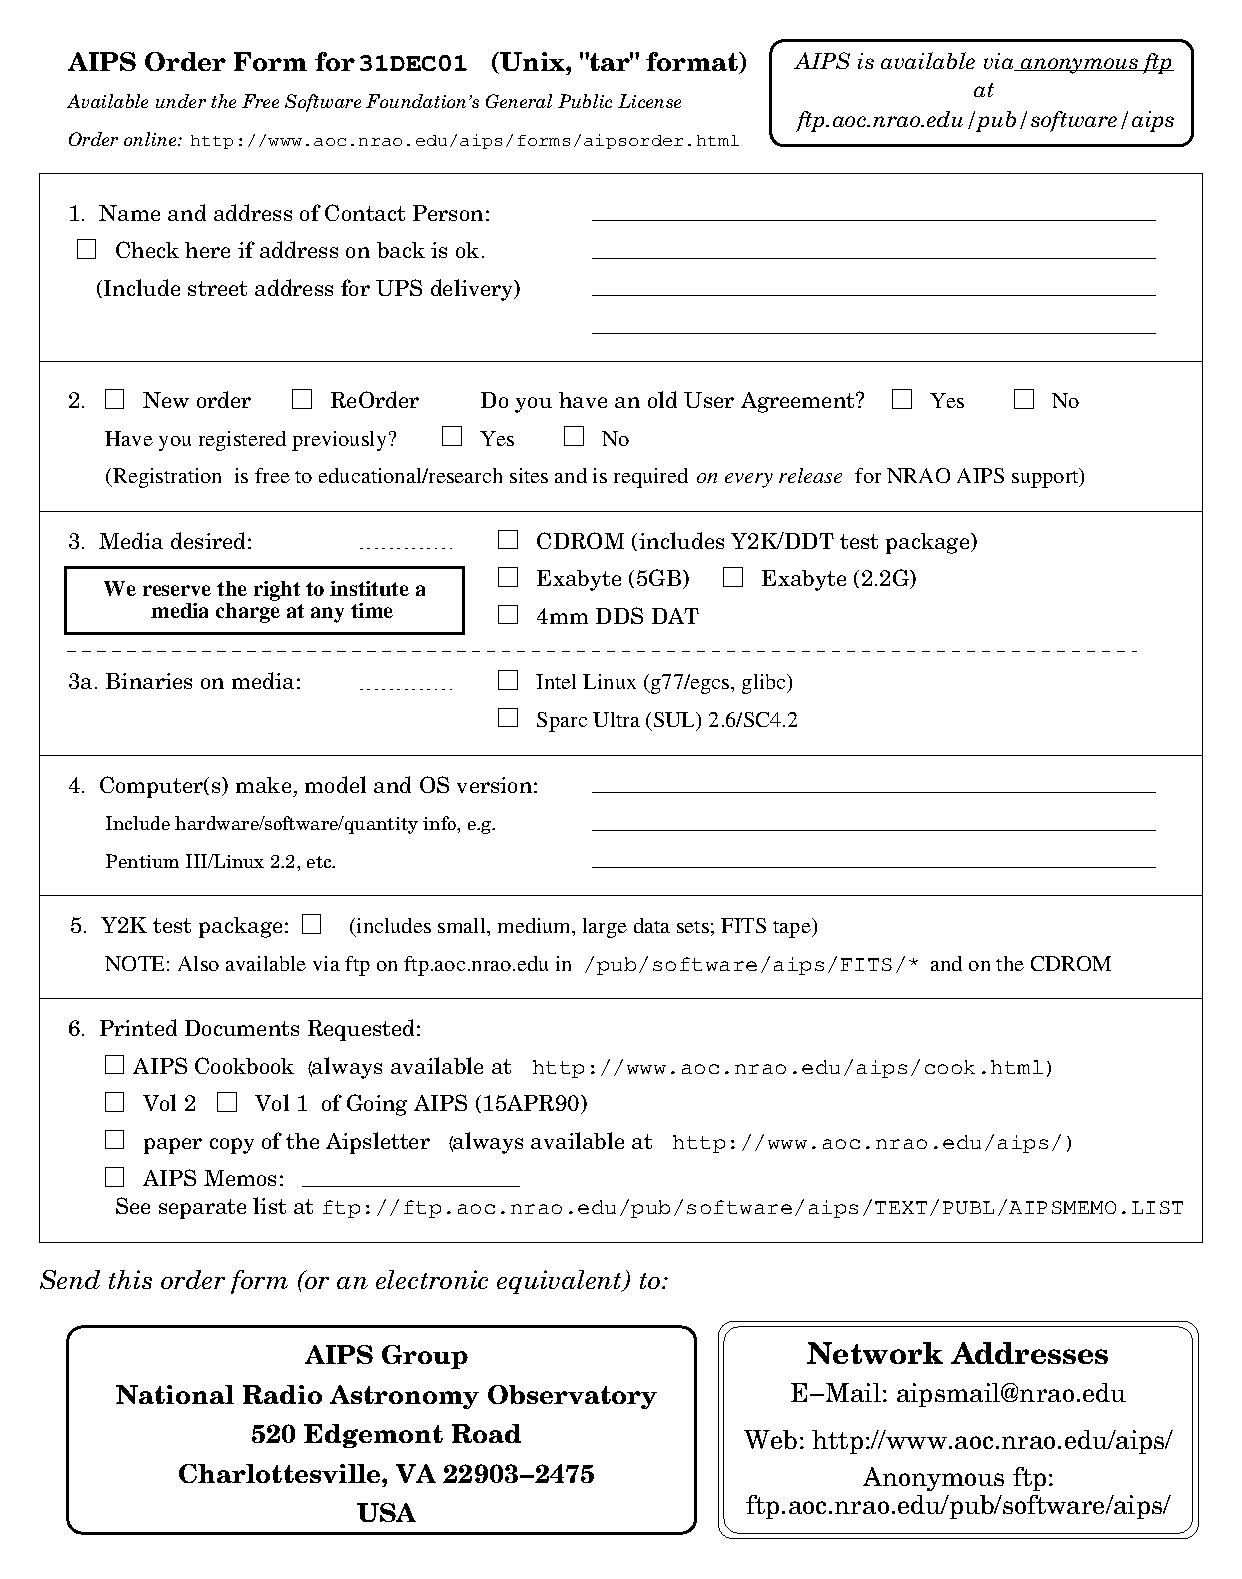
\includegraphics{FIG/AIPSORDER.PS}}}
%\vfill\eject
\vbox to 4.4in{
\vspace{12pt}
%\centerline{\rotatebox{-90}{\resizebox{!}{3.5in}{%
%\includegraphics{FIG/Mandrill.color.plt}}}}
\centerline{\resizebox{!}{3.5in}{\includegraphics{FIG/Mandrill.eps}}}
\vspace{12pt}
\centerline{{\huge \tt \AIPRELEASE}}
\vspace{12pt}
\vfill}
\phantom{...}
\centerline{\resizebox{!}{!}{\includegraphics{FIG/AIPSLETS.PS}}}

\end{document}
